\documentclass[]{article}
\usepackage{amsmath}
\usepackage{amssymb}
\usepackage{subcaption}
\usepackage{graphicx}
\usepackage{float}
\usepackage{multicol}


%\usepackage{easyReview} %used for annotation. Cannot be run together with (changes) - command "highlight" defined twice
\usepackage{changes}%use while actively annotating

%\usepackage[final]{changes} % once we are happy with all annotation, we can accept all proposed changes and show only the final document.

% simply select text you want to annotate and start typing the command \replacedGM{the selected text will appear here}{and here you enter the new replacement text}
\definechangesauthor[name={Timo}, color=orange]{tp}
\definechangesauthor[name={Giovanni}, color=green]{gm}
\newcommand{\replacedTP}[2]{\replaced[id=tp]{#2}{#1}}
\newcommand{\addedTP}[1]{\added[id=tp]{#1}}
\newcommand{\deletedTP}[1]{\deleted[id=tp]{#1}}
\newcommand{\highlightTP}[1]{\highlight[id=tp]{#1}}
\newcommand{\commentTP}[2]{\comment[id=tp]{#2}{#1}}

\newcommand{\replacedGM}[2]{\replaced[id=gm]{#2}{#1}}
\newcommand{\addedGM}[1]{\added[id=gm]{#1}}
\newcommand{\deletedGM}[1]{\deleted[id=gm]{#1}}
\newcommand{\highlightGM}[1]{\highlight[id=gm]{#1}}
\newcommand{\commentGM}[2]{\comment[id=gm]{#2}{#1}}

%opening
\title{}
\author{}

\begin{document}
	
	\maketitle
	
	
\section*{Question 4: CS Regression}
\subsection*{a. replication of Cochrane's graph 15.1 and 15.2}
	
\begin{figure}[h]
	\begin{subfigure}{0.5\textwidth}
		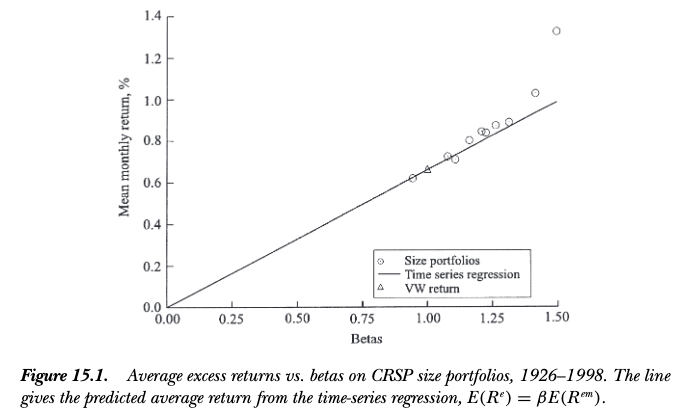
\includegraphics[width=1\linewidth, height=6cm]{Cochrane_15_1} 
		\caption{15.1}
		\label{fig:subim1}
	\end{subfigure}
	\begin{subfigure}{0.5\textwidth}
		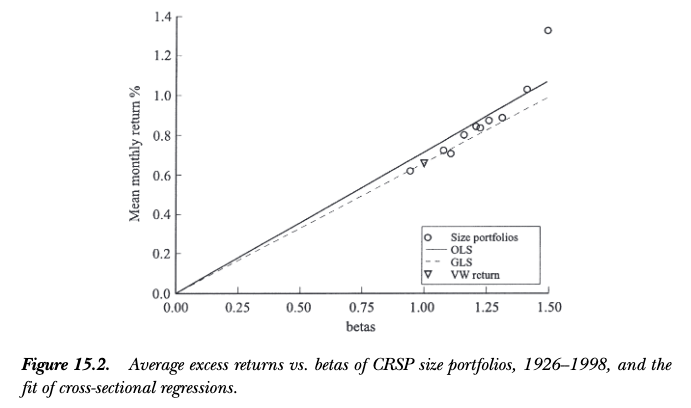
\includegraphics[width=1\linewidth, height=6cm]{Cochrane_15_2}
		\caption{15.2}
		\label{fig:subim2}
	\end{subfigure}	
	\caption{The original figures from Cochrane, 2005}
	\label{fig:image1}
\end{figure}

Replication of 15.1 time series regression $E(R^{ei}) = \beta E(R^{em})$. Set-up of data acquisition and regression analysis:

\begin{itemize}
	\item using the R package "frenchdata", download value weighted, size sorted portfolio returns and factors, join tables,
	\item filter data on 1926-1998 time frame,
	\item for each decile calculate excess return $R^{ei} = R^{i} - R_{f}$
	\item for each decile, regress $E[R^{ei}] = \beta_i E[R^{me}]$
	\item plot $E[R^{ei}]$ on $\beta_i$
\end{itemize}

In the data, we find 12 monthly timeseries consisting of i=1,..,10 size sorted portfolios, the test assets $R^{i}$, the excess return of the market $R^{me}=R^m - R_f$ and the risk-free rate $R_f$. The factor pricing model $R_t^{ei}=\alpha_i + \beta_i f_t+e^i$ prices the excess return on the test assets on the factor f, the excess return on the market. The model expected returns $E(R^{ei})=\beta_iE(f)$ imply:
\begin{itemize}
	\item $E(e^i)=0$. In fact $e\sim N(0,\Omega)$.
	\item $E(R^{ei})$ are linear in the $\beta_i$.
	\item By $E(e^i)=0$, the model pricing errors accumulate in the regression intercepts $\alpha_i$, with expectation $E(\alpha_i)=0$.
	\item Given that the factor is an excess return and given that the market portfolio is an investable asset it is also priced by the model. $E(R^{me}) = \beta E(R^{me})$ holds with $\beta=1$. The factor risk premium is therefore simply $\hat{\lambda}=1 E(R^{me}) = E_T(f)$.
\end{itemize}

The expected excess return-beta timeseries model is fit in graph 15.1 precisely on two points $(\beta, R^e)$:
\begin{itemize}
	\item The market excess return $(1, E_T(f)=E(R^{me}))$ as outlined above and
	\item The risk-free and therefore certain risk-free rate $(0, R_f=0)$. 
\end{itemize}

The slope of the model matches the expected factor risk premium $\hat{\lambda} = \frac{E_T(f)-0}{1-0}$. The vertical distances between the model line and the test assets represent the pricing error $\alpha_i$.

It is observed that the smallest size-decile exhibits the largest mean monthly excess return as well as estimated $\beta$. The positive pricing error is largest for the smallest size-decile, but smaller than in the original Cochrane figures. The reason for this is unclear, but may be related to adjustments applied on the dataset by French after 2009, or related to data adjustments that were adopted by French but not by Cochrane or vice versa.

\begin{figure}[H]
	\begin{subfigure}{0.5\textwidth}
		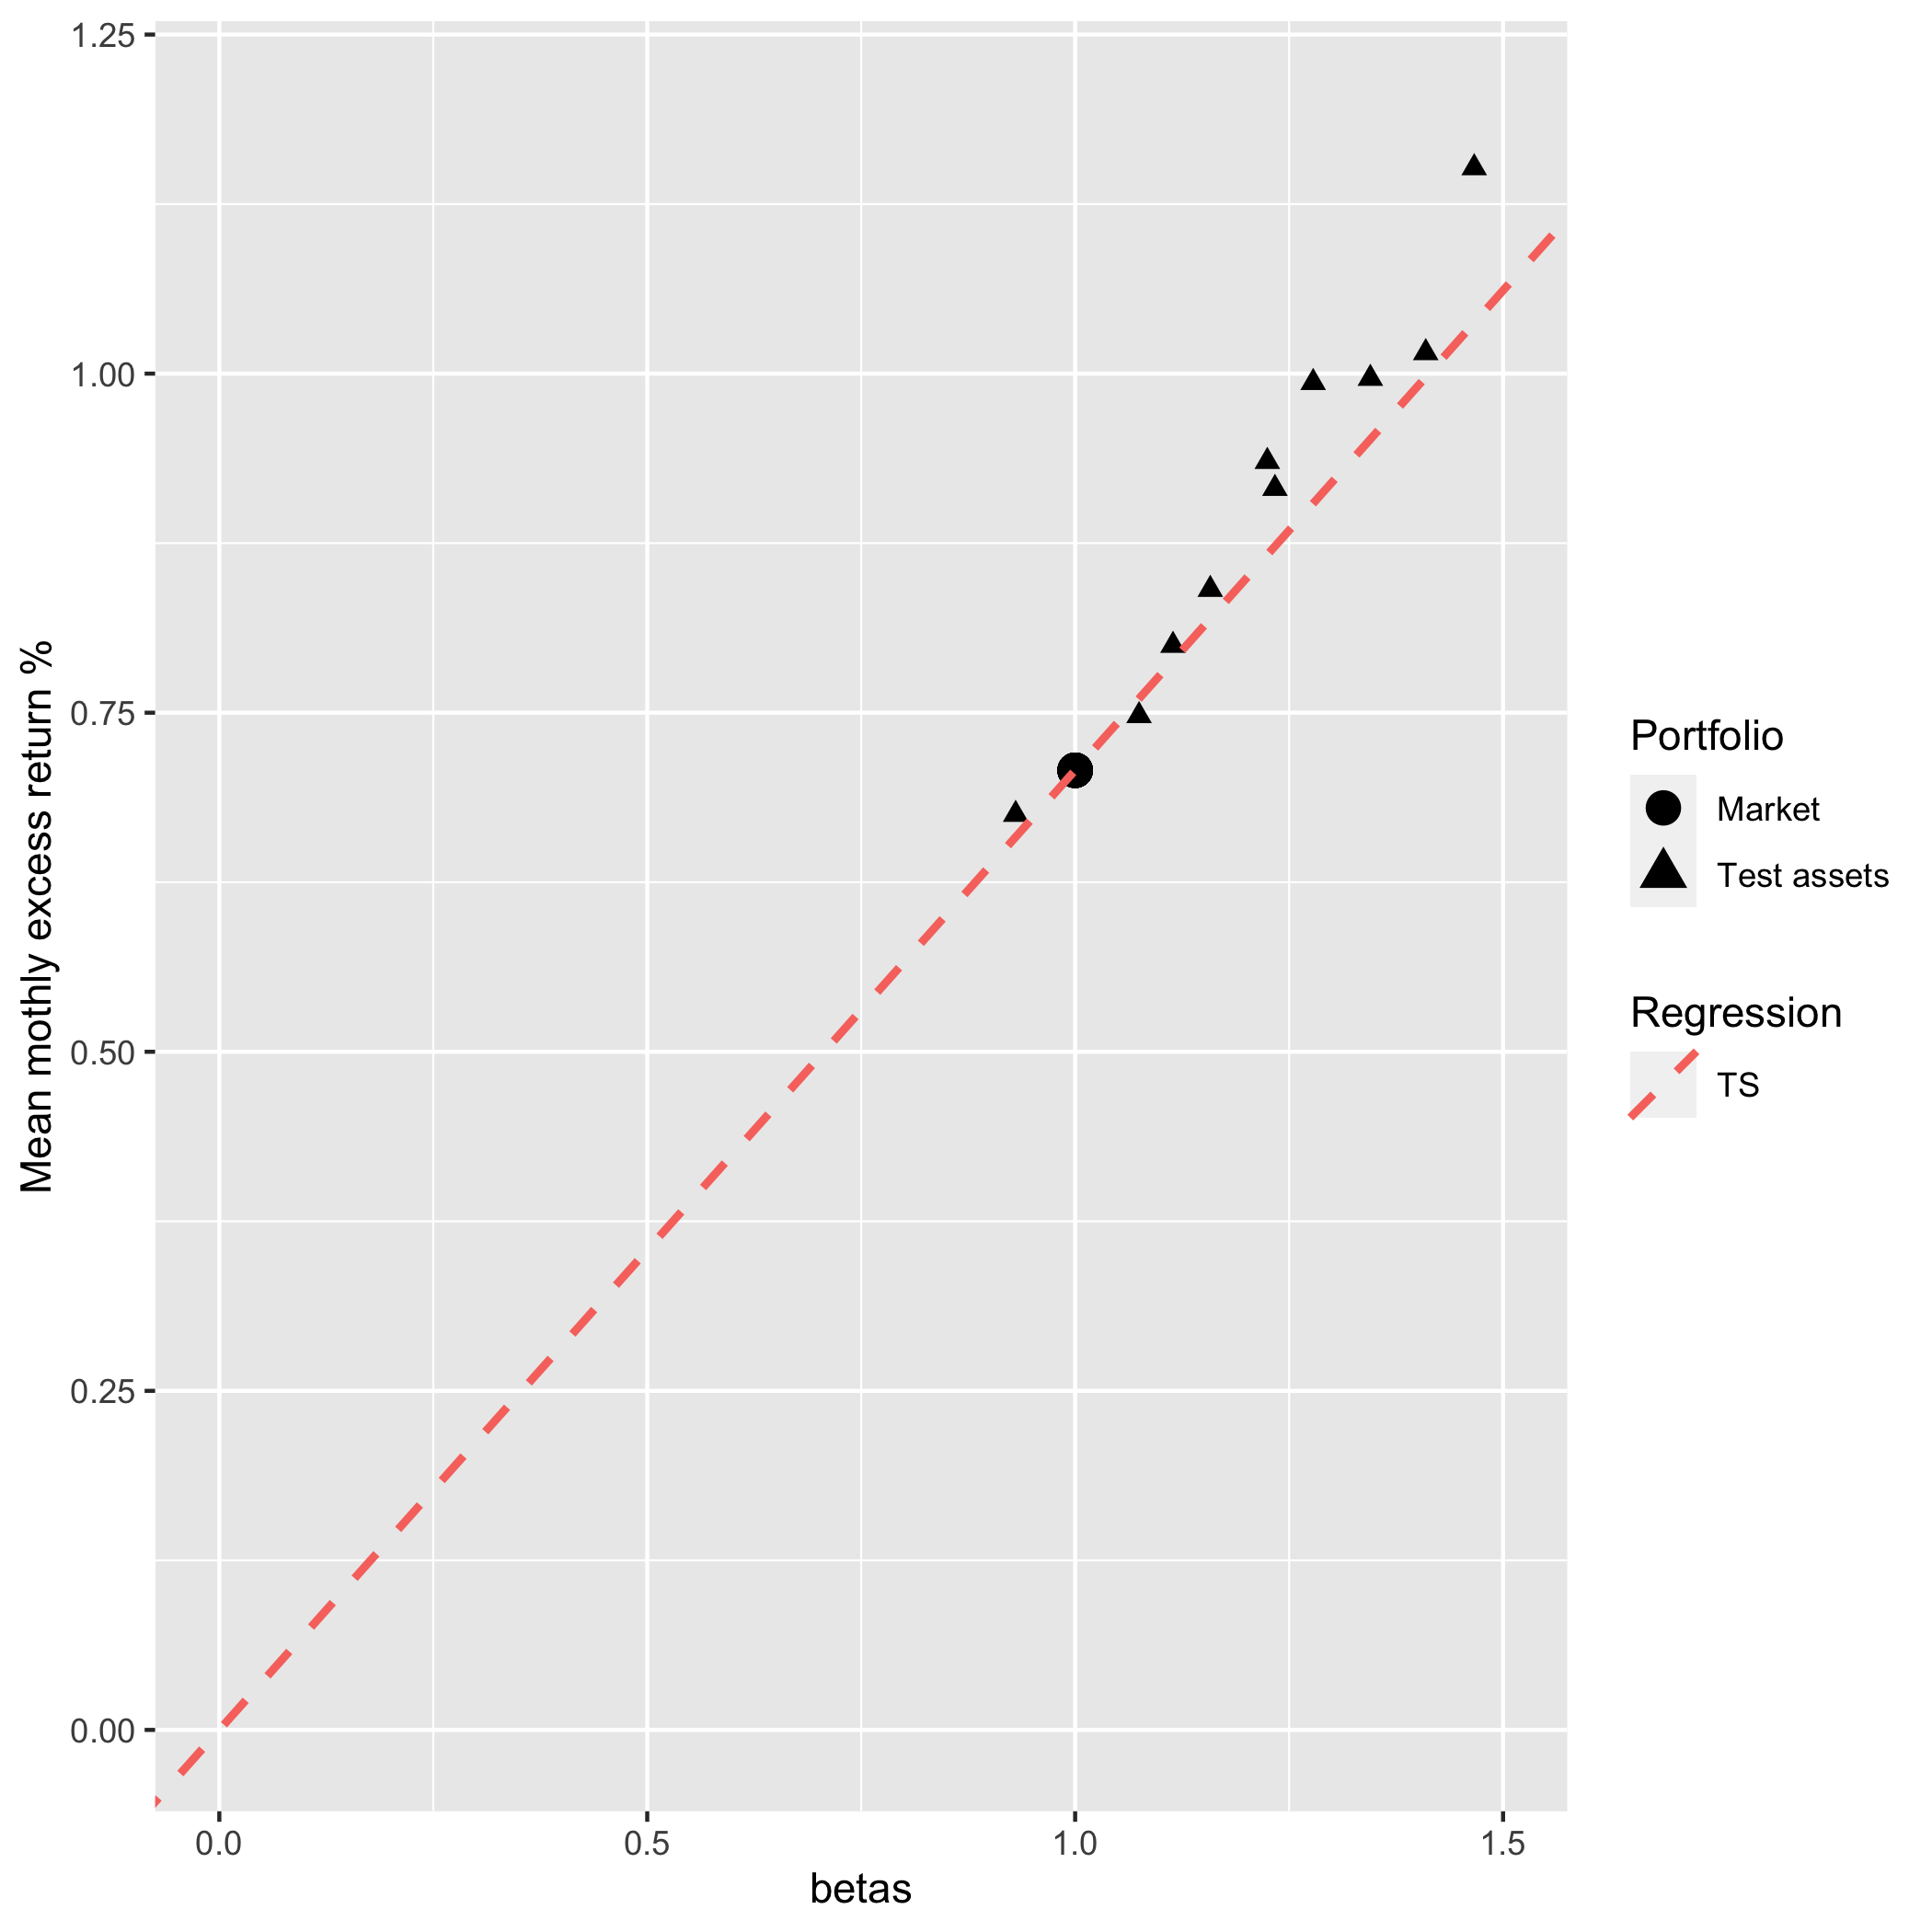
\includegraphics[width=1\linewidth, height=6cm]{replicated_15_1} 
		\caption{15.1}
		\label{fig:subim3}
	\end{subfigure}
	\begin{subfigure}{0.5\textwidth}
		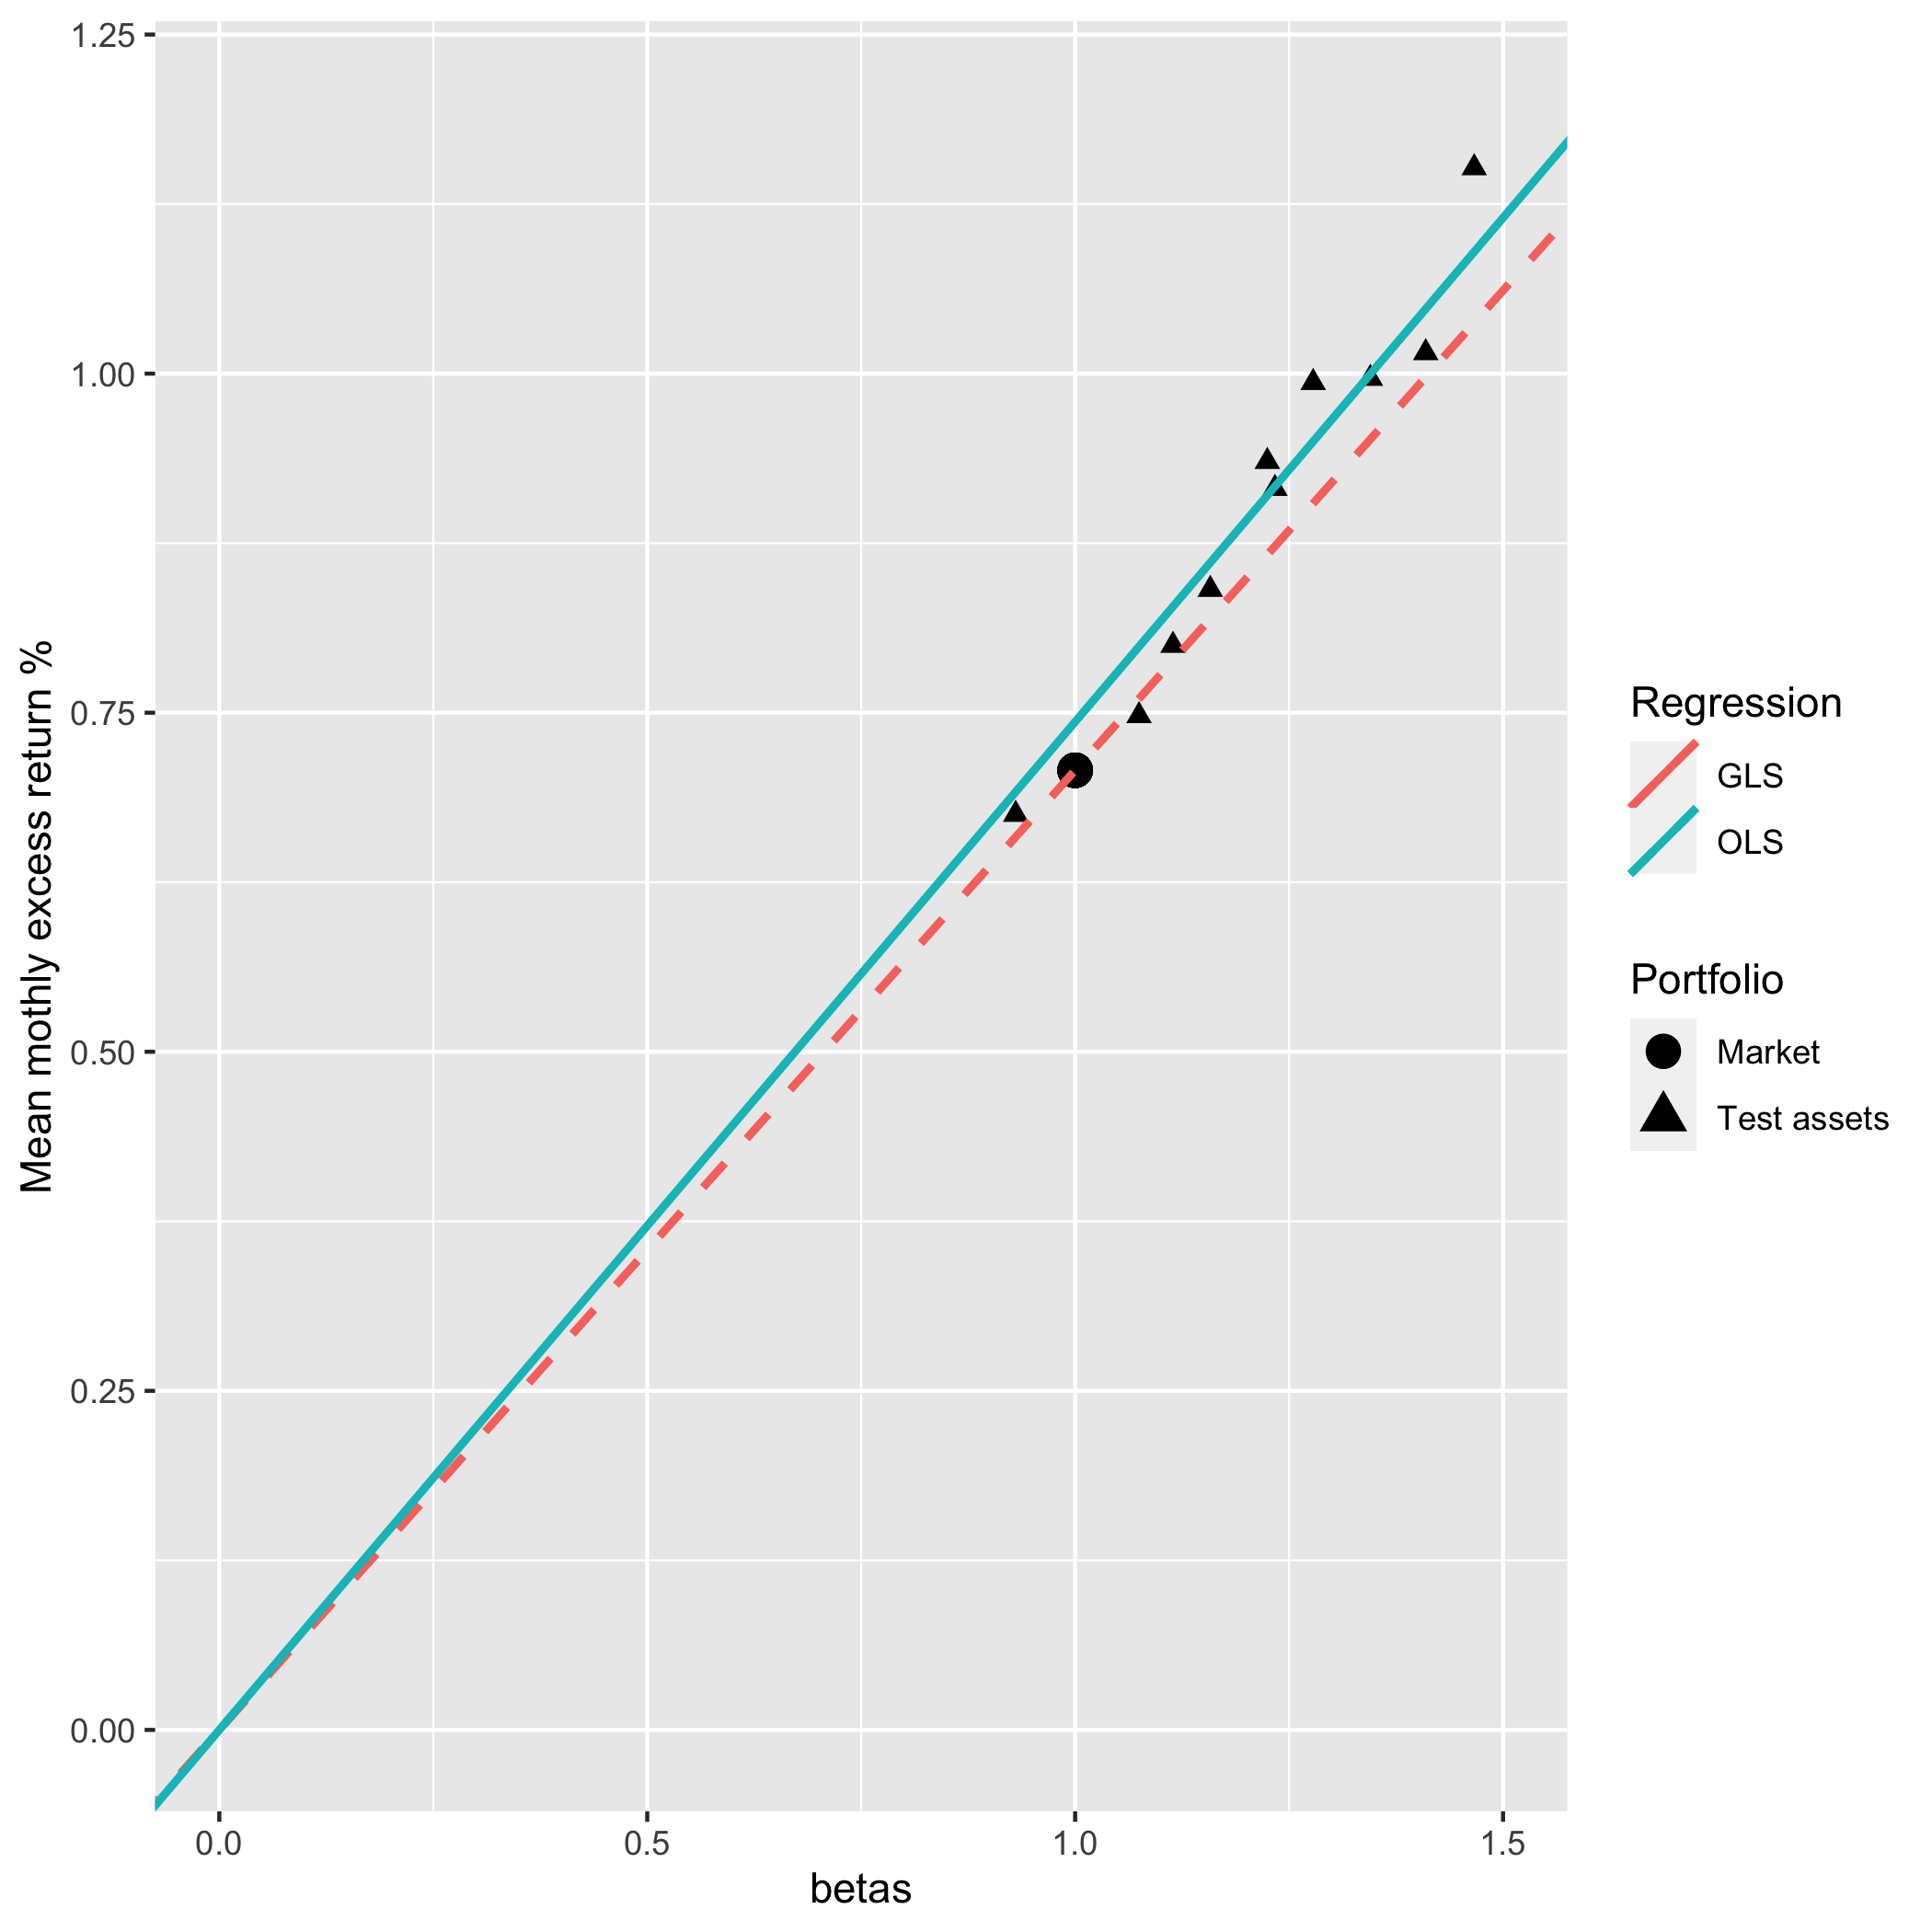
\includegraphics[width=1\linewidth, height=6cm]{replicated_15_2}
		\caption{15.2}
		\label{fig:subim4}
	\end{subfigure}	
	\caption{The original figures from Cochrane, 2005}
	\label{fig:image2}
\end{figure}
	
\subsection*{What do these figures tell us about the CAPM?}	
The largest pricing error in the TS regression occur in the smallest size-decile. This is the the small firm anomaly or size premium and is considered a failure of the CAPM. Numerous attempts were made to explain this anomaly: Banz (1981) suggests that small firms face larger cost of capital than large firms which may explain an incentive to merge and form conglomerates. The size effect has been reproduced for numerous sample periods and for most major securities markets around the world (Hawawini and Keim, 2000). However, it tends to be weaker internationally, e.g., Crain (2011) and Bryan (2014). A number of sub-effects have been noted, such as the January-effect, whereby the size premium is observed particularly in the first trading days of the year and is largely absent the rest of the year Reinganum (1981), Roll (1981), Keim (1983), Gu (2003), Easterday, Sen, and Stephan (2009). Additonally, the size effect appears to have weakened significantly since it was first detected in the early 1980s e.g., Dichev (1998), Chan, Karceski, and Lakonishok (2000), Horowitz, Loughran and Savin (2000), Amihud (2002), Schwert (2003) and Van Dijk (2011). The size effect appears to be driven by "extreme" stocks. Removing stocks with less than USD 5m in market cap or alternatively the smallest 5\% of firms causes the small firm effect to vanish e.g., Horowitz, Loughran, and Savin (2000), Crain (2011) and Bryan (2014). Additionally, Crain (2011) suggests that size may be a proxy for liquidity. Controlling for firm quality, a robust size effect emerges according to "Size Matters, If You Control Your Junk" by Assness, Frazzini, Israel, Mosksowitz, and Pedersen (2015). Quality stocks are safe, profitable, growing, and well managed. Quality is measured using the Quality Minus Junk (QMJ) factor proposed by Asness, Frazzini, and Pedersen (2014). This is just a short review of attempts to explain the size or small firm anomaly and the extensive research on this topic undertaken after Cochrane produced the figures 15.1 and 15.2 in 2005 may explain why the K. French dataset evolved and now controls for some of the above listed effects.

\section*{b. testing the CAPM}
\subsection*{Replicate the first 3 columns in Table 15.1, and the first 4 columns of Table  15.2 of  Cochrane  (2005,  book)}

Estimates of $\hat{\lambda}$
\begin{itemize}
	
	\item \textbf{TimeSeries Estimate $\hat{\lambda_{TS}}$} A first stage ols timeseries regression 
	
	\begin{align}\label{1stage}
		R_t^{ei}=\alpha_i+\beta_i f_t+e^i
	\end{align}
	
	See code line 120: ols\_model generates estimates of $\alpha_i$ and $\beta_i$ for each test asset. As outlined above, given that the factor is an excess return itself and given that the market portfolio is an investable asset it is also priced by the model. The factor risk premium is therefore simply $$\hat{\lambda_{TS}}=1 E(R^{me}) = E_T(f)$$ which is estimated using the second stage cross sectional regression 
	
	\begin{align}
		E(R^{ei})=\beta_i'\lambda + \alpha_i
	\end{align}
	
	\item \textbf{Cross Sectional Estimate $\hat{\lambda}$} Using the $\beta_i$ 	and the regression residuals $e^i$ obtained from (\ref{1stage}), the estimators for $\hat{\lambda}$ and their standard errors are derived. 
	
	\begin{tabular}{|l|l|l|l|}
		\hline
		Estimator & TS & OLS & GLS \\
		\hline
		$\hat{\lambda}$&$E_T(f)$&$(\beta'\beta)^{-1}\beta'E(R^e)$&$\left(\beta'\Sigma^{-1}\beta\right)^{-1}\beta'\Sigma^{-1}E_T(R^)e$\\
		$\sigma^2(\lambda)$ &  &   $\left[\frac{1}{T}(\beta'\beta)^{-1}\Sigma\beta(\beta'\beta)^{-1}+\Sigma_f\right]$  & $\frac{1}{T}\left[(\beta'\Sigma^{-1}\beta)^{-1}+\Sigma_f\right]$ \\
		$SE_{\lambda}$ &  &   $\sqrt{\left[\frac{1}{T}(\beta'\beta)^{-1}\Sigma\beta(\beta'\beta)^{-1}+\Sigma_f\right]}$  & $\sqrt{\frac{1}{T}\left[(\beta'\Sigma^{-1}\beta)^{-1}+\Sigma_f\right]}$ \\
		\hline
	\end{tabular}
	
	Cochrane tests the robustness of the estimation results by varying the assumptions about the distribution of the regression residuals and the residual covariance matrix $\Sigma$. The covariance matrix of the factor $\Sigma_f$ is a scalar and not affected by these variations.
	
	\begin{tabular}{|l|l|l|}
		\hline
		Assumption & Description& $\Sigma$\\
		\hline
		i.i.d &$\sigma^2_i = e_i^2 = \sigma^2 \ \forall i=1..N, E(e_ie_j)=0 \forall i \ne j$ & $\sigma^2I_T$\\
		0-lag & $\sigma^2_i = e_i^2, E(e_ie_j)=0 \forall i \ne j$  & $\sigma_t^2I_T$\\
		3-lag-NW&heteroskedasticity and auto-correlation   &\\
		24-lag&&\\
		\hline
	\end{tabular}
	
	need to distinguish between
	\begin{itemize}
		\item SE w/ and w/o Shanken correction\\
		\item p-values for finite sample, and asymptotic distributions\\
		\item Which  are  these  distributions?Write  their names and the number(s) of degrees of freedom.
		\item Does  the  Shanken  correction  change  the  results?
		\item Repeat the above analyses in question (a) and (b) on the extended sample: 1926.01 to 2021.12, and by adding the 12 industry portfolios of Fama and French.
		\item Do the results change by adding new test assets?
		\item What do these Tables tell us about the CAPM?
		
	\end{itemize}
	
	Having obtained estimates for 
	
	\begin{tabular}{|l|l|l|l|}
		\hline
		Estimator & TS & OLS & GLS \\
		\hline
		$\hat{\lambda}$&$E_T(f)$&$(\beta'\beta)^{-1}\beta'E(R^e)$&$\left(\beta'\Sigma^{-1}\beta\right)^{-1}\beta'\Sigma^{-1}E_T(R^)e$\\
		$\sigma^2(\lambda)$ &  &   $\left[\frac{1}{T}(\beta'\beta)^{-1}\Sigma\beta(\beta'\beta)^{-1}+\Sigma_f\right]$  & $\frac{1}{T}\left[(\beta'\Sigma^{-1}\beta)^{-1}+\Sigma_f\right]$ \\
		$cov(\hat{\alpha})$&&$\frac{1}{T}\left[I-\beta(\beta'\beta)\beta'\right]\Sigma\left[I-\beta(\beta'\beta)\beta'\right]'$&$\frac{1}{T}\left[\Sigma-\beta(\beta'\Sigma^{-1}\beta)^{-1}\beta'\right]$\\
		\hline
	\end{tabular}
	
\end{itemize}



\end{document}